\documentclass[11pt,a4paper]{article}
\usepackage[utf8]{inputenc}
\usepackage[T1]{fontenc}
\usepackage[polish]{babel}
\usepackage{amsmath,amssymb}
\usepackage{graphicx}
\usepackage{booktabs}
\usepackage{hyperref}
\usepackage{float}
\usepackage{geometry}
\usepackage{fancyhdr}
\geometry{margin=2.5cm}

\pagestyle{fancy}
\fancyhf{}
\lhead{MPUM}
\chead{\textbf{Miniprojekt 1}}
\rhead{Mateusz Wojaczek}
\cfoot{\thepage/\pageref{LastPage}}
\usepackage{lastpage}

\begin{document}

\begin{center}
{\Large\textbf{Miniprojekt 1 -- Regresja liniowa}}\\[0.3em]
{\large Metody probabilistyczne w uczeniu maszynowym}\\[0.3em]
Mateusz Wojaczek
\end{center}

\section*{Streszczenie}

W tym raporcie opisuję implementację regresji liniowej na danych z pliku \texttt{dane.data} -- 8~cech wejściowych i jedna zmienna objaśniana. Zacząłem od prostego modelu liniowego, potem testowałem różne funkcje bazowe (wielomiany, funkcje gaussowskie, Fouriera, sigmoidalne), regularyzacje L1, L2 i Elastic Net. Całość zaimplementowałem od zera w~NumPy, bez gotowych bibliotek ML.

\section{Przygotowanie danych}

\subsection{Wczytywanie i podział}

Dane wczytuję z pliku \texttt{dane.data}. Przy każdym uruchomieniu losuję kolejność obserwacji, a następnie dzielę je na trzy zbiory w proporcji $0.6 : 0.2 : 0.2$ (treningowy, walidacyjny, testowy). Hiperparametry dobieram na zbiorze walidacyjnym, a ostateczną ocenę modelu robię na zbiorze testowym.

\subsection{Standaryzacja}

Przed trenowaniem standaryzuję cechy wejściowe -- od każdej cechy odejmuję jej średnią i dzielę przez odchylenie standardowe (oba liczone na zbiorze treningowym). Zbiory walidacyjny i testowy transformuję tymi samymi parametrami co treningowy. Zmiennej~$y$ nie skaluję.


\subsection{Analiza korelacji}

Na ustandaryzowanych danych policzyłem macierz korelacji Pearsona. Widać z niej kilka rzeczy:
\begin{itemize}
    \item Cechy $x_2$ i $x_7$ są ekstremalnie silnie skorelowane.
    \item Zmienna $y$ jest najsilniej skorelowana z cechami $x_1$, $x_4$ i $x_5$.
    \item Pozostałe cechy ($x_3$, $x_6$, $x_8$) mają słabszą korelację z~$y$.
\end{itemize}

\begin{figure}[H]
    \centering
    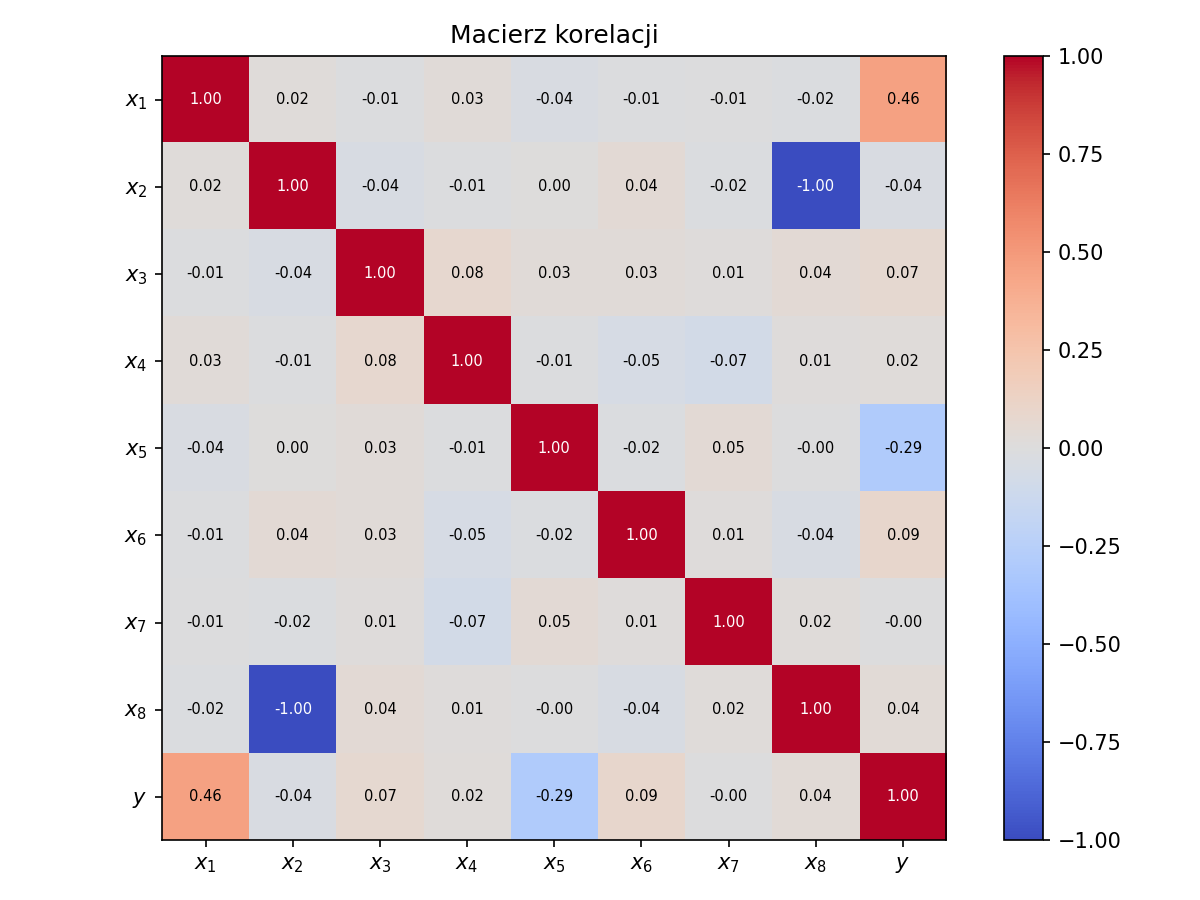
\includegraphics[width=0.6\textwidth]{images/correlation_matrix.png}
    \caption{Macierz korelacji między cechami a zmienną objaśnianą}
\end{figure}

\section{Model liniowy -- rozwiązanie analityczne}

Zacząłem od najprostszego modelu: regresja liniowa z funkcjami bazowymi $\varphi(x) = [1, x_1, \ldots, x_8]$, kwadratowa funkcja straty:
$$\ell(\theta) = \frac{1}{m}\sum_{i=1}^{m}(\hat{y}^{(i)} - y^{(i)})^2$$

Rozwiązanie analityczne to $\theta = (X^TX + \lambda I)^{-1}X^Ty$, gdzie $I$ ma wyzerowany element $(0,0)$ żeby nie regularyzować biasu. Dla $\lambda \to 0$ dostałem:

\begin{center}
    \textbf{Train MSE: 10602.69 \quad Test MSE: 11440.03}
\end{center}

\subsection{Wpływ regularyzacji L2 na rozwiązanie analityczne}

Sprawdziłem jak zmienia się MSE przy różnych wartościach $\lambda$ w regularyzacji grzbietowej:

\begin{table}[H]
\centering
\begin{tabular}{rrr}
\toprule
$\lambda$ & Train MSE & Test MSE \\
\midrule
$10^{-6}$ & 10602.65 & 11436.51 \\
0.1       & 10602.65 & 11436.55 \\
0.5       & 10602.65 & 11436.69 \\
1         & 10602.66 & 11436.86 \\
5         & 10602.73 & 11438.32 \\
10        & 10602.95 & 11440.26 \\
50        & 10609.61 & 11460.23 \\
100       & 10628.40 & 11494.63 \\
1000      & 11514.92 & 12546.28 \\
\bottomrule
\end{tabular}
\caption{MSE rozwiązania analitycznego dla różnych $\lambda$ (regularyzacja L2)}
\end{table}

Widać, że przy małych $\lambda$ regularyzacja praktycznie nie zmienia wyniku, a przy dużych wartościach model jest za bardzo ograniczony i MSE rośnie. W przypadku prostego modelu liniowego regularyzacja nie daje poprawy.

\section{Metody gradientowe}

\subsection{Gradient descent (pełny)}

Zaimplementowałem klasyczny gradient descent z learning rate $\eta = 0.01$. Warunek stopu: albo ustalone $k$ iteracji, albo norma różnicy $\theta$ poniżej progu $10^{-6}$. Gradient kwadratowej funkcji straty:
$$\nabla\ell(\theta) = \frac{2}{m}X^T(X\theta - y)$$

Przy 1000 iteracjach gradient ładnie zbiega do zera, a MSE stabilizuje się.

\begin{figure}[H]
    \centering
    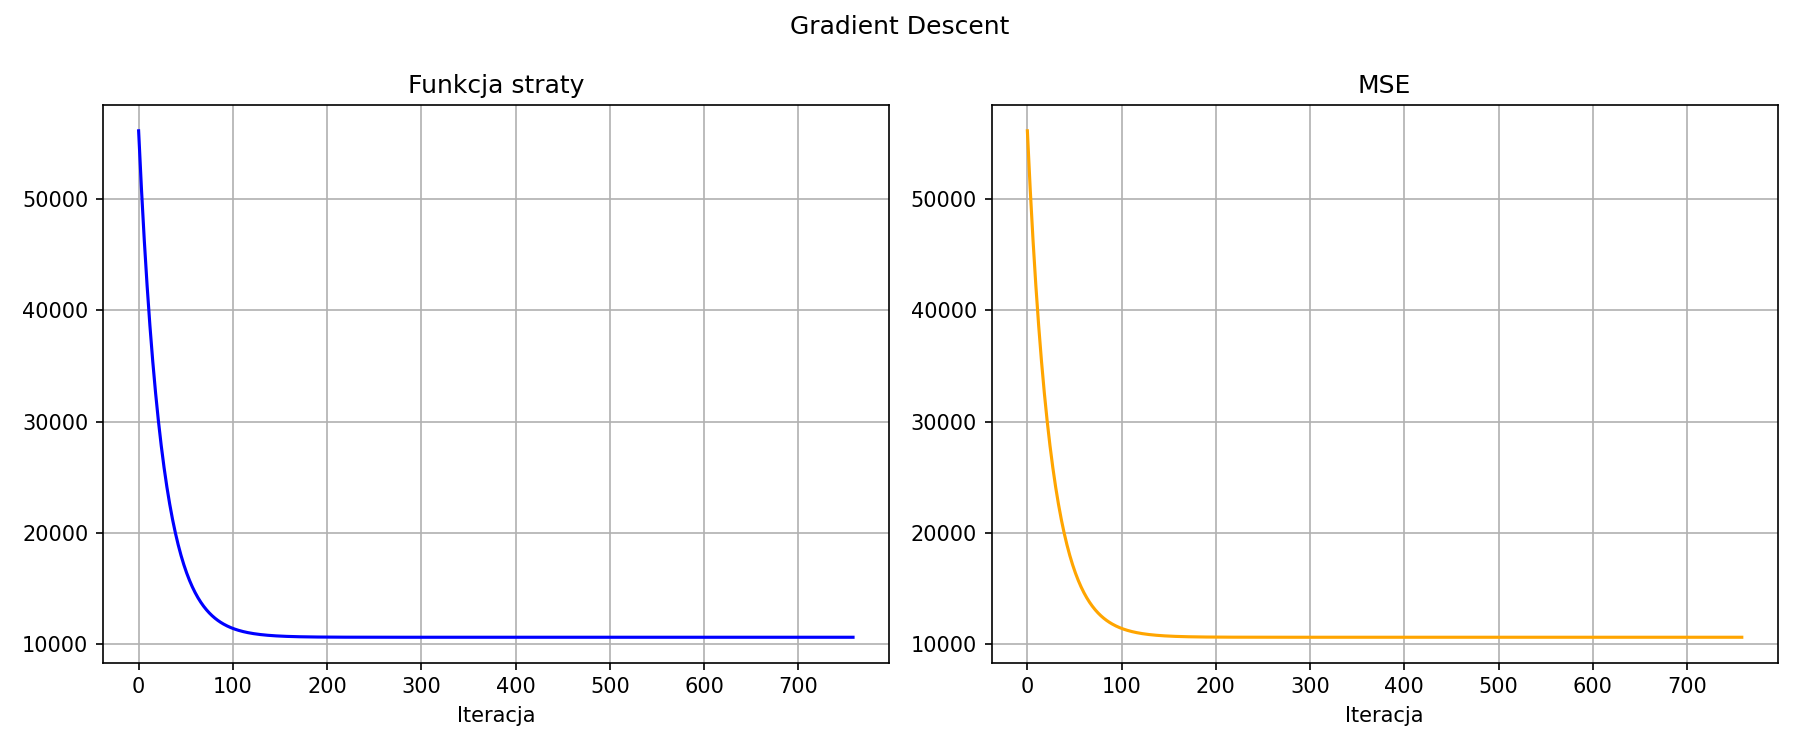
\includegraphics[width=0.85\textwidth]{images/gd_training.png}
    \caption{Gradient i MSE w kolejnych iteracjach -- pełny gradient descent}
\end{figure}

\subsection{Mini-batch gradient descent}

Zaimplementowałem też wersję mini-batch. Przetestowałem różne rozmiary batchy: 1, 8, 16, 32.

\begin{figure}[H]
    \centering
    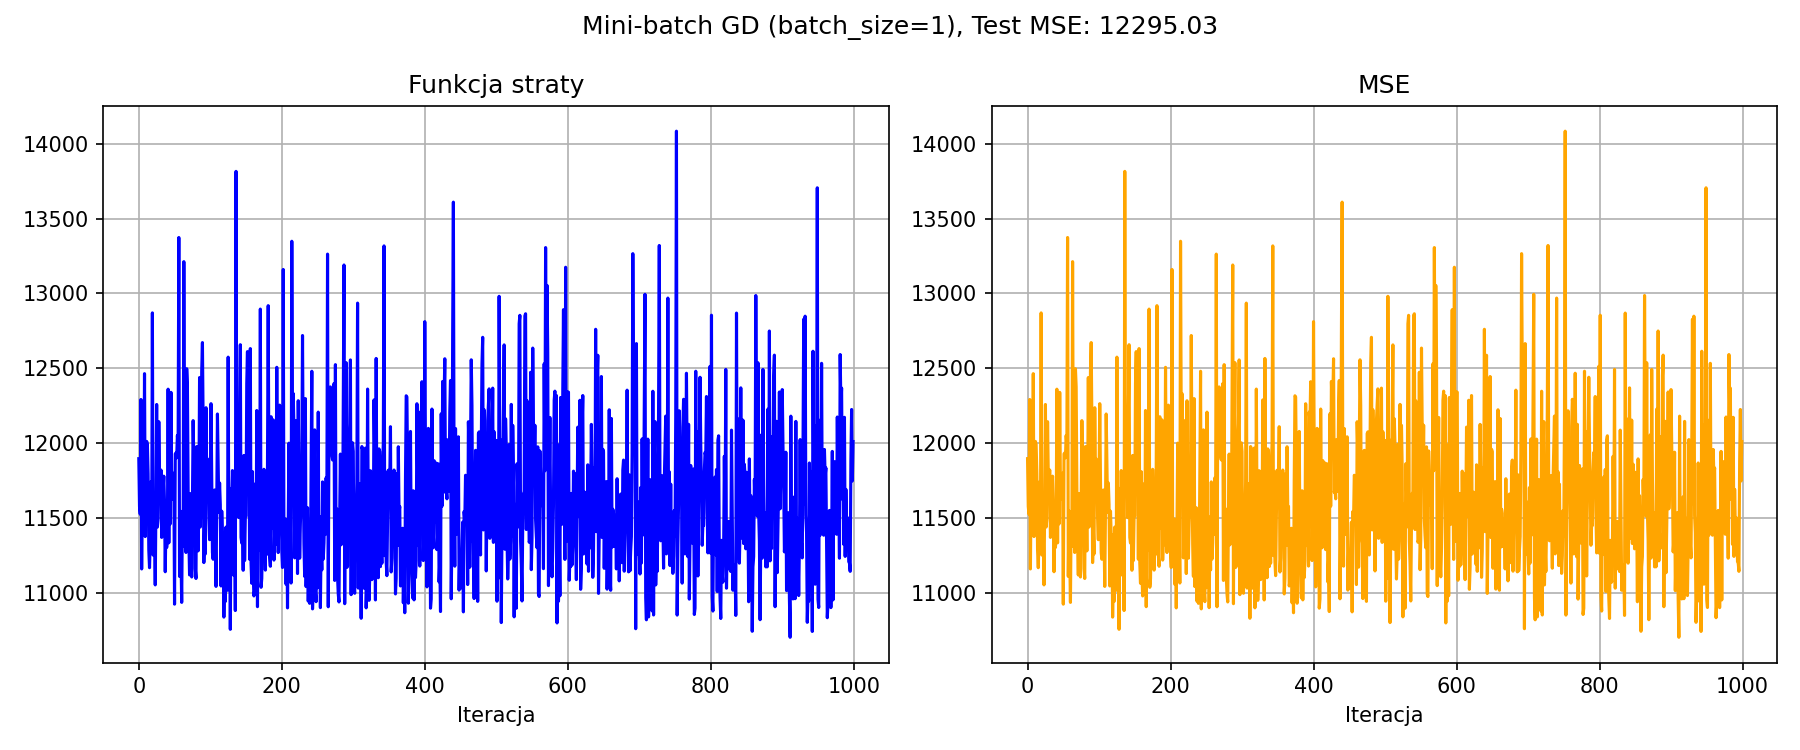
\includegraphics[width=0.48\textwidth]{images/minibatch_1.png}
    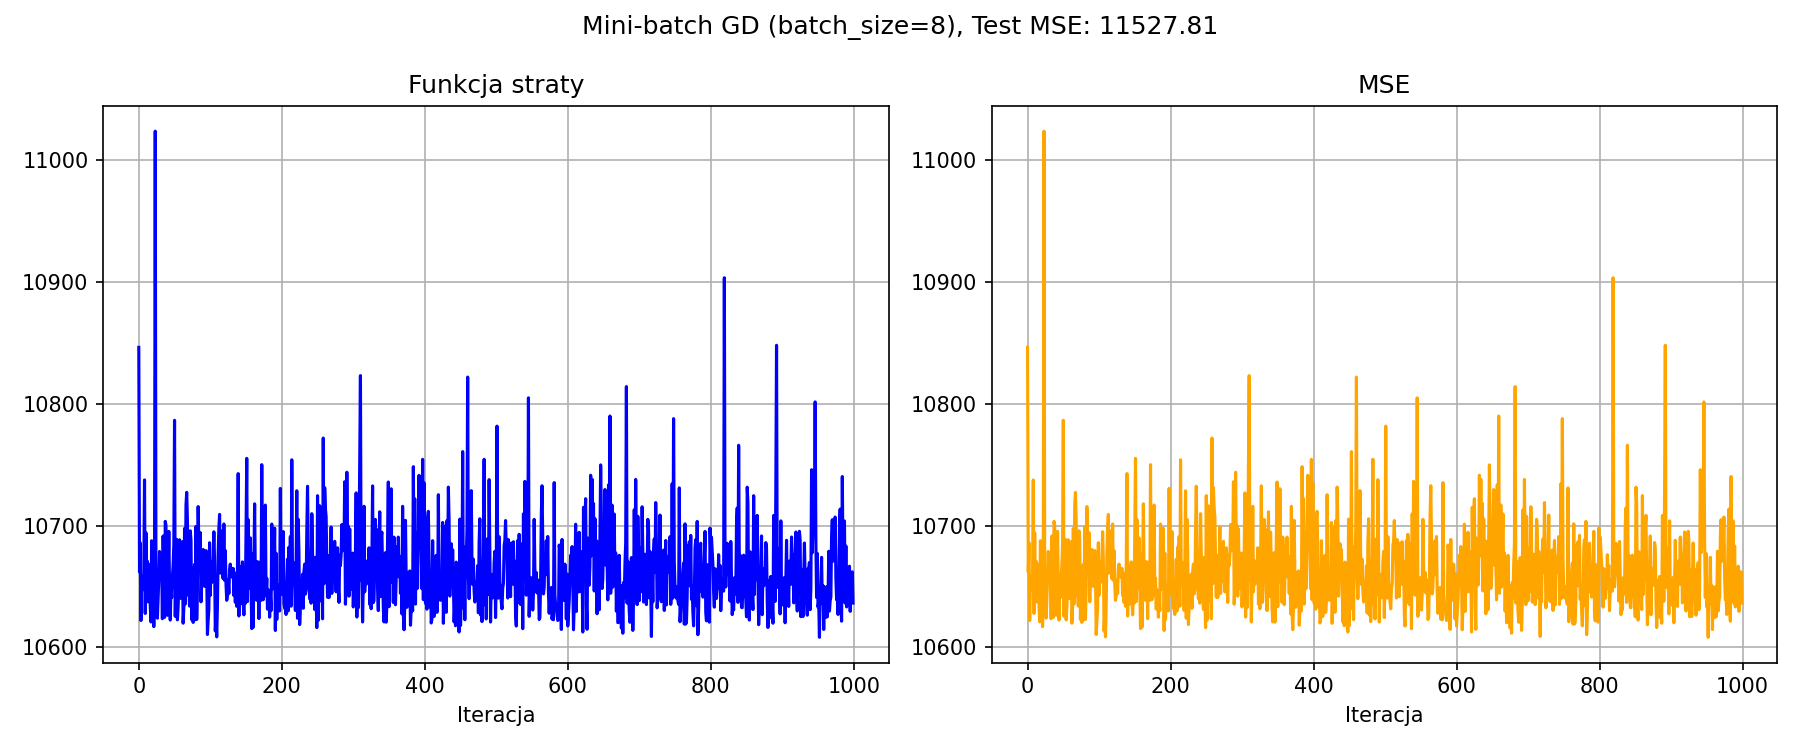
\includegraphics[width=0.48\textwidth]{images/minibatch_8.png}\\[0.5em]
    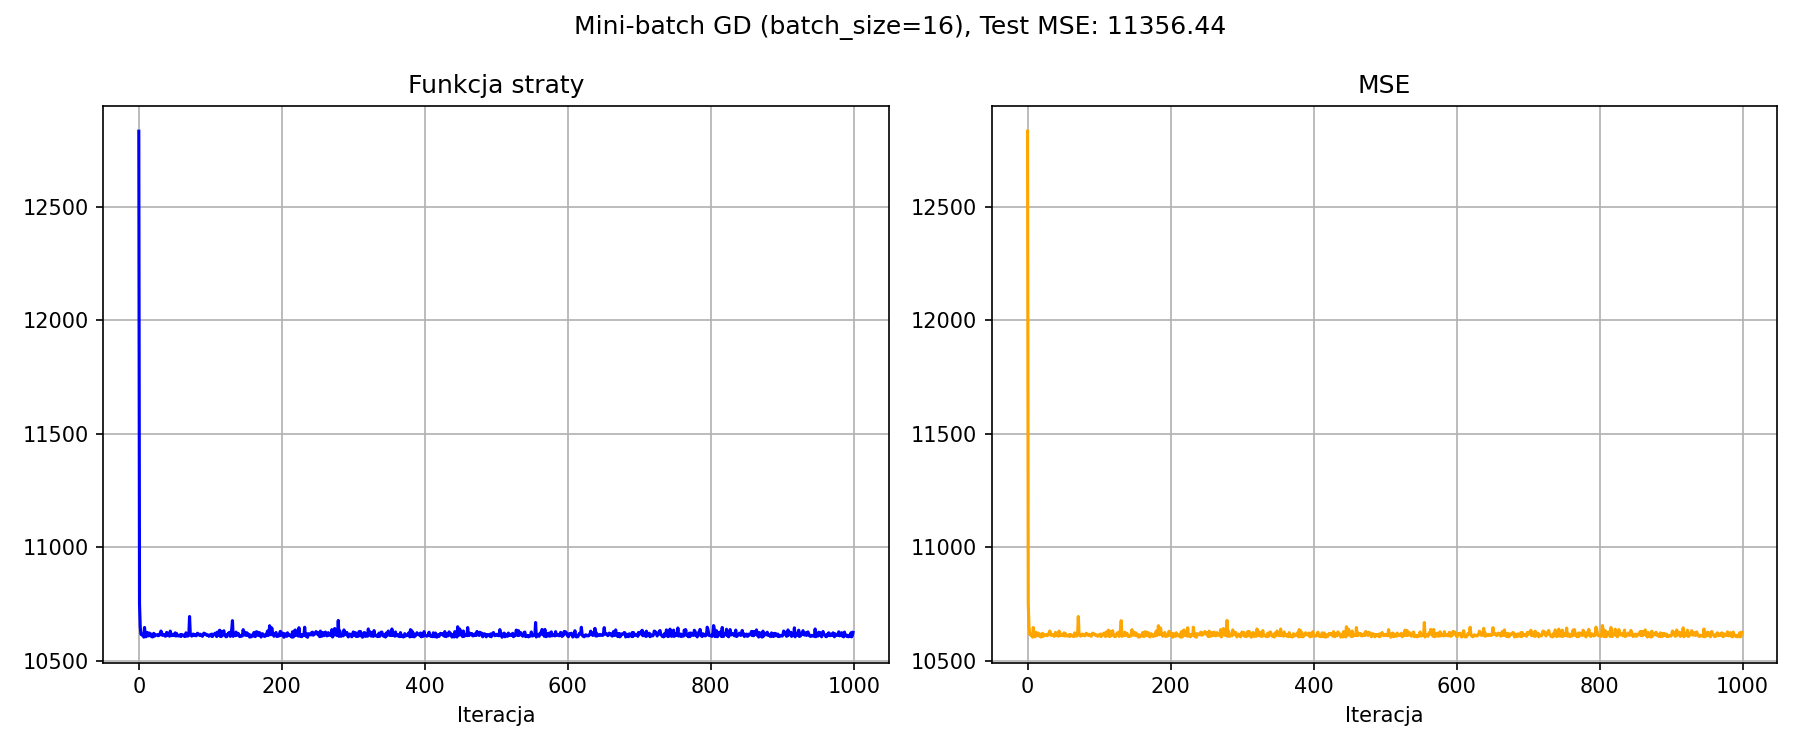
\includegraphics[width=0.48\textwidth]{images/minibatch_16.png}
    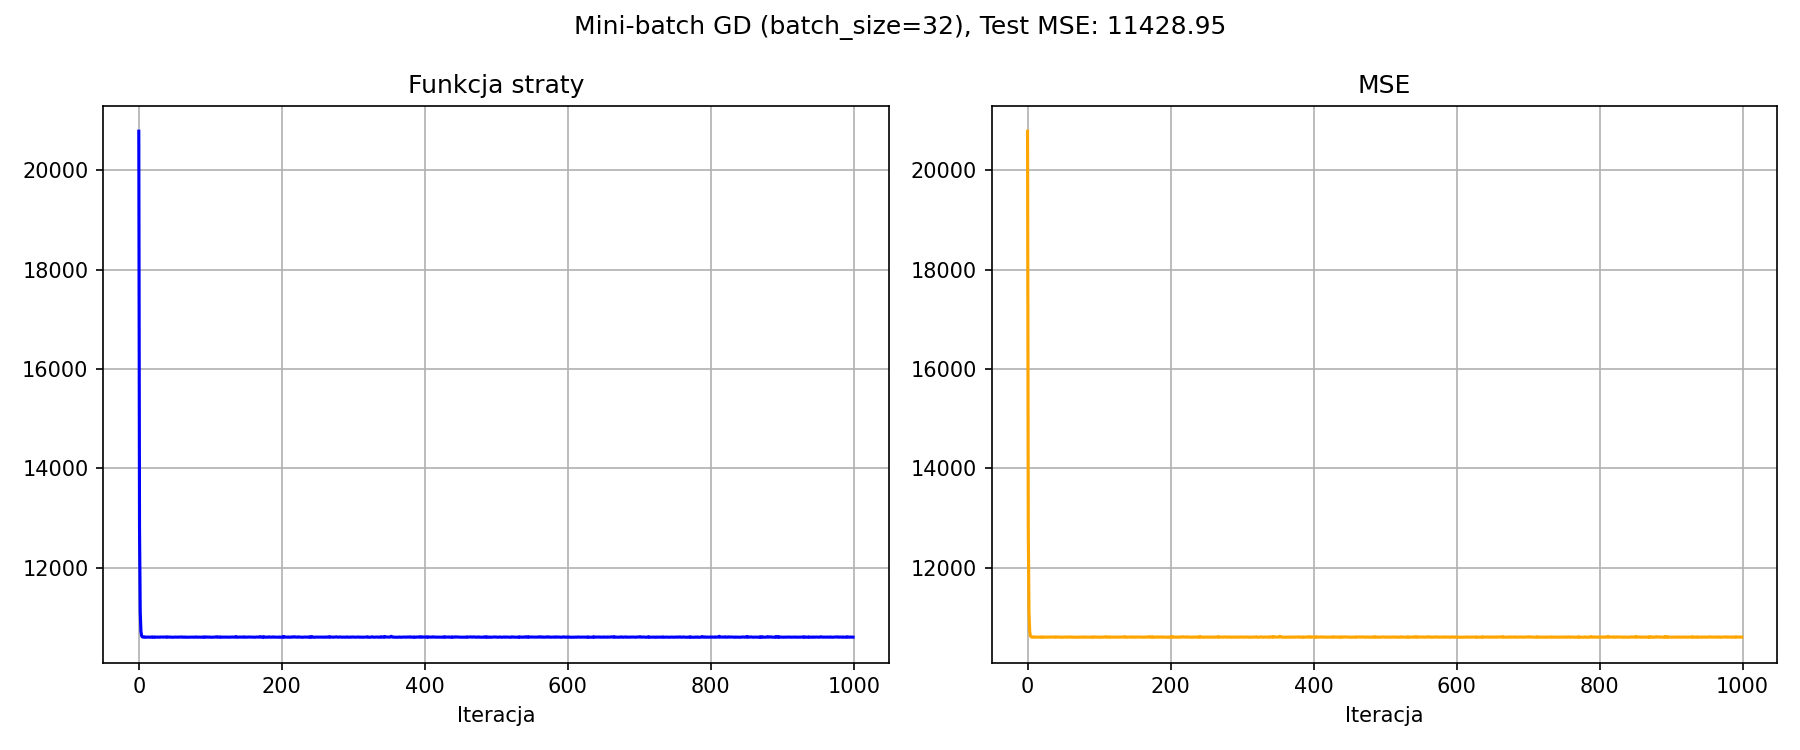
\includegraphics[width=0.48\textwidth]{images/minibatch_32.png}
    \caption{Mini-batch gradient descent dla różnych rozmiarów batcha}
\end{figure}

Przy mini-batchu gradient nie zbiega gładko do zera, tylko oscyluje -- to normalne, bo w~każdej iteracji liczymy gradient na losowym podzbiorze danych. Mimo to model uczy się poprawnie, a cały proces jest znacznie szybszy niż pełny GD.

\section{Regularyzacja -- dobór hiperparametrów}

Do wyznaczenia parametrów regularyzacji użyłem zbioru walidacyjnego. Testowałem wartości $\lambda \in \{0, 0.0001, 0.001, 0.002, 0.005, 0.01, 0.02, 0.05, 0.1, 1, 2, 5, 10\}$.

\subsection{Regularyzacja L1 (Lasso)}

Do gradientu dodaję składnik $\lambda_1 \cdot \mathrm{sign}(\theta)$ (z pominięciem biasu).

\begin{figure}[H]
    \centering
    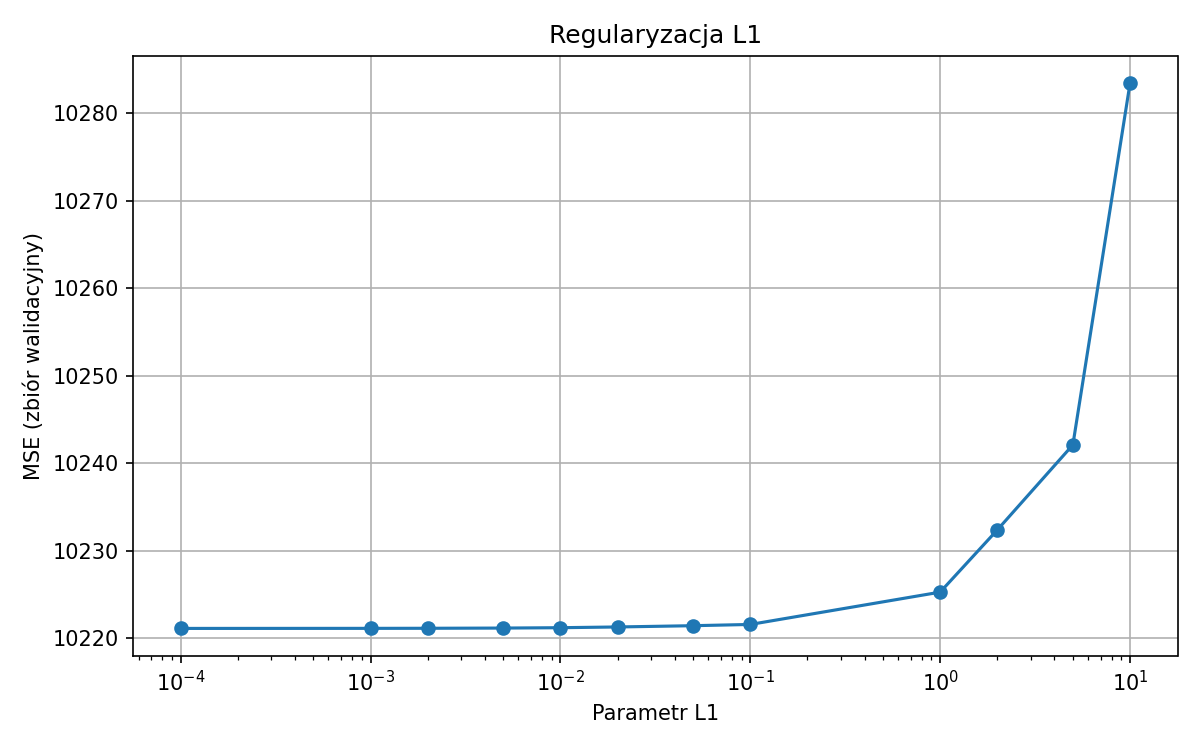
\includegraphics[width=0.55\textwidth]{images/l1_regularization.png}
    \caption{MSE na zbiorze walidacyjnym dla różnych parametrów L1}
\end{figure}

\subsection{Regularyzacja L2 (Ridge)}

Do gradientu dodaję składnik $2\lambda_2 \cdot \theta$ (bez biasu).

\begin{figure}[H]
    \centering
    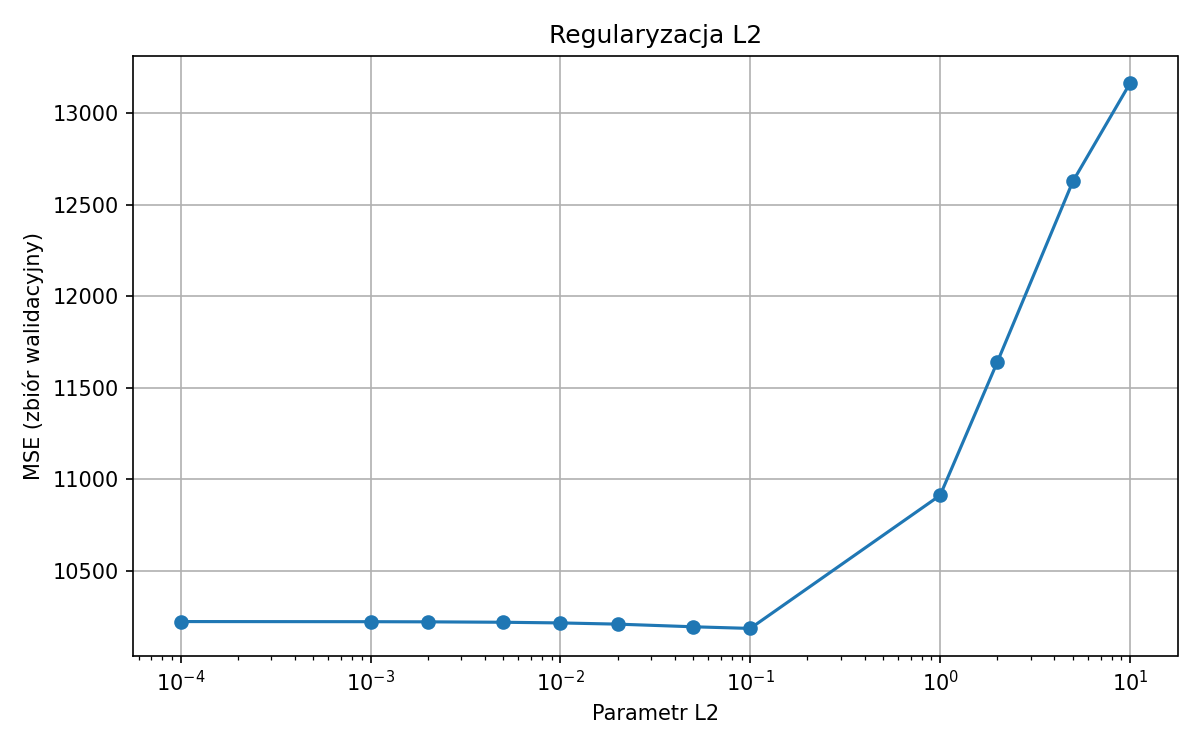
\includegraphics[width=0.55\textwidth]{images/l2_regularization.png}
    \caption{MSE na zbiorze walidacyjnym dla różnych parametrów L2}
\end{figure}

\subsection{Elastic Net (L1 + L2)}

Przetestowałem kombinacje L1 i L2 -- pełen grid $\lambda_1 \times \lambda_2$. Najlepsze parametry to $\lambda_1 = 0$, $\lambda_2 = 0.1$ z MSE = 10183.48 na zbiorze walidacyjnym. W przypadku prostego modelu liniowego regularyzacja nie przynosi dużej poprawy.

\section{Funkcje bazowe}

Tu zaczyna się najciekawsza część. Zamiast modelować $y$ jako kombinację liniową surowych cech, transformuję cechy przez funkcje bazowe i dopiero na wyniku robię regresję liniową.

\subsection{Wielomiany}

Klasa \texttt{Polynomial(degree)} generuje cechy $[1, x_1, \ldots, x_8, x_1^2, \ldots, x_8^2, \ldots, x_1^d, \ldots, x_8^d]$. Testowałem stopnie od 1 do 5.

\begin{figure}[H]
    \centering
    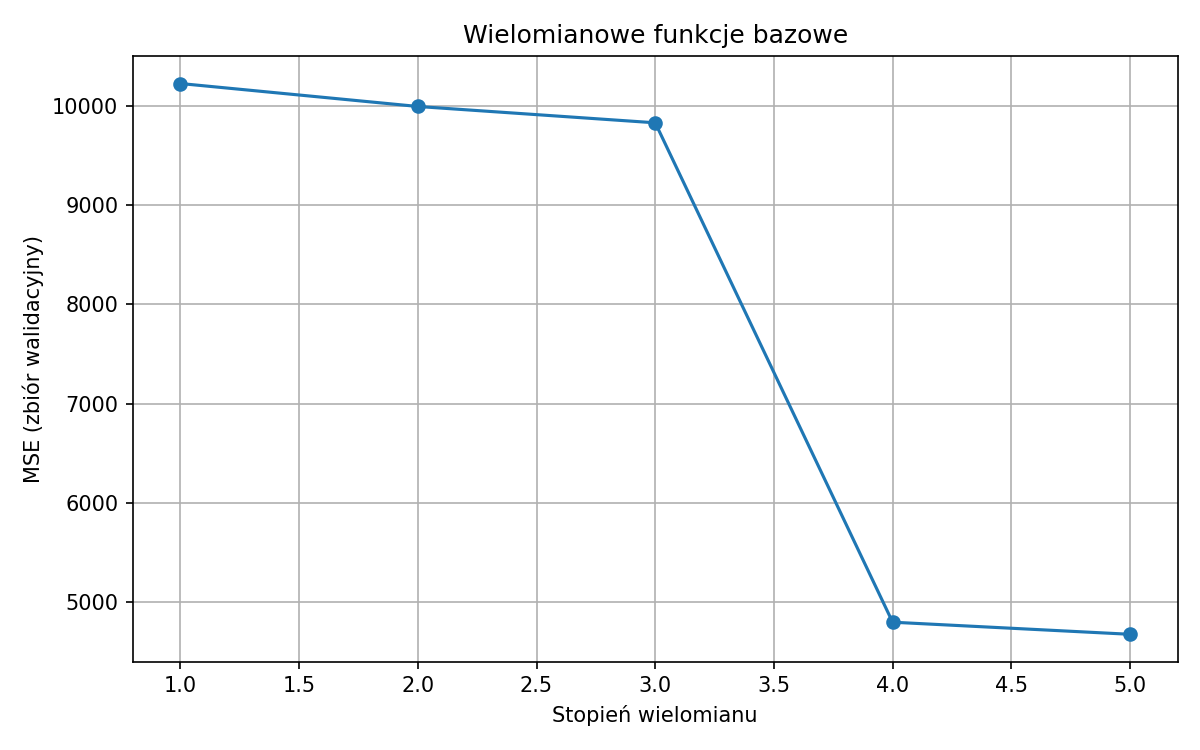
\includegraphics[width=0.55\textwidth]{images/polynomial_comparison.png}
    \caption{MSE na zbiorze walidacyjnym dla różnych stopni wielomianu}
\end{figure}

Najlepszy wynik dał wielomian stopnia 5 -- Test MSE: \textbf{4942.57}. To ogromna poprawa w~stosunku do modelu liniowego (11440).

\subsection{Funkcje gaussowskie}

Dla każdej cechy generuję funkcje postaci $\exp\left(-\frac{(x - \mu)^2}{2\sigma^2}\right)$, gdzie $\mu$ to centra rozłożone równomiernie w zakresie danych. Testowałem różne wartości $\sigma$.

\begin{figure}[H]
    \centering
    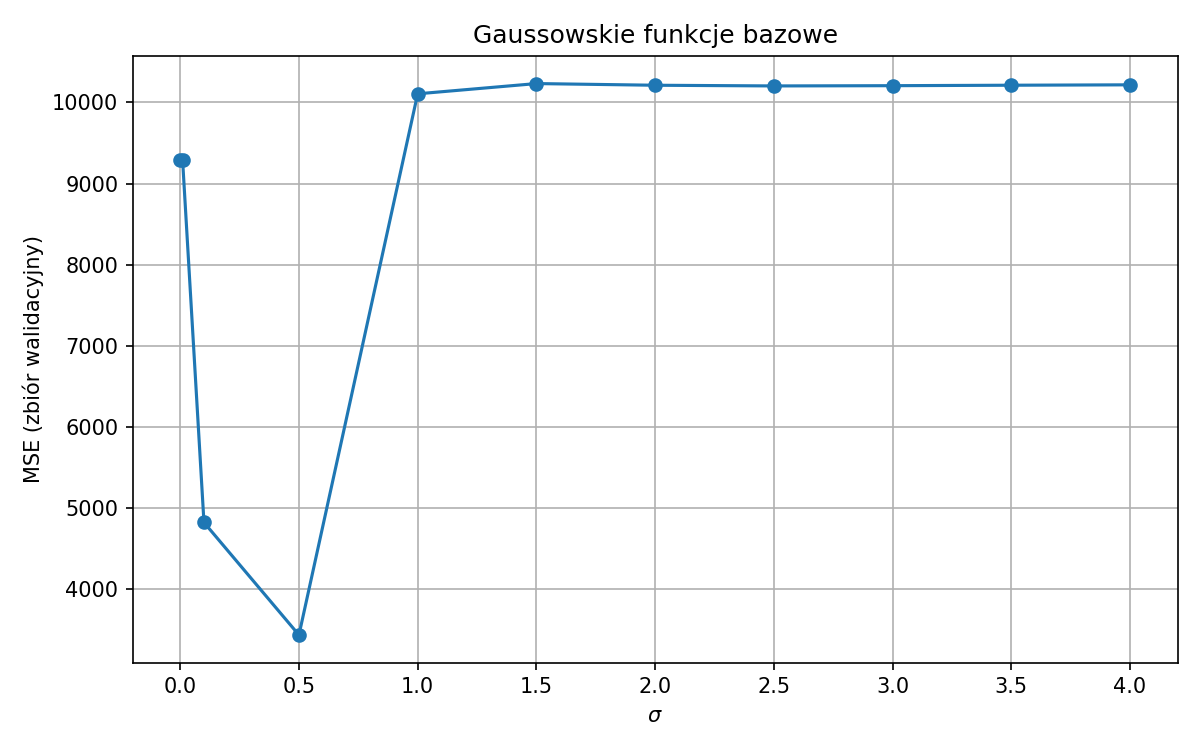
\includegraphics[width=0.55\textwidth]{images/gaussian_comparison.png}
    \caption{MSE na zbiorze walidacyjnym dla różnych $\sigma$ funkcji gaussowskiej}
\end{figure}

Najlepsza gaussowska (połączona z cechami liniowymi, $\sigma = 0.5$) dała Test MSE: \textbf{4042.12}.

\subsection{Funkcje Fouriera}

Generuję cechy $[\sin(2\pi k x), \cos(2\pi k x)]$ dla $k = 1, \ldots, n$. Testowałem różne częstotliwości.

\begin{figure}[H]
    \centering
    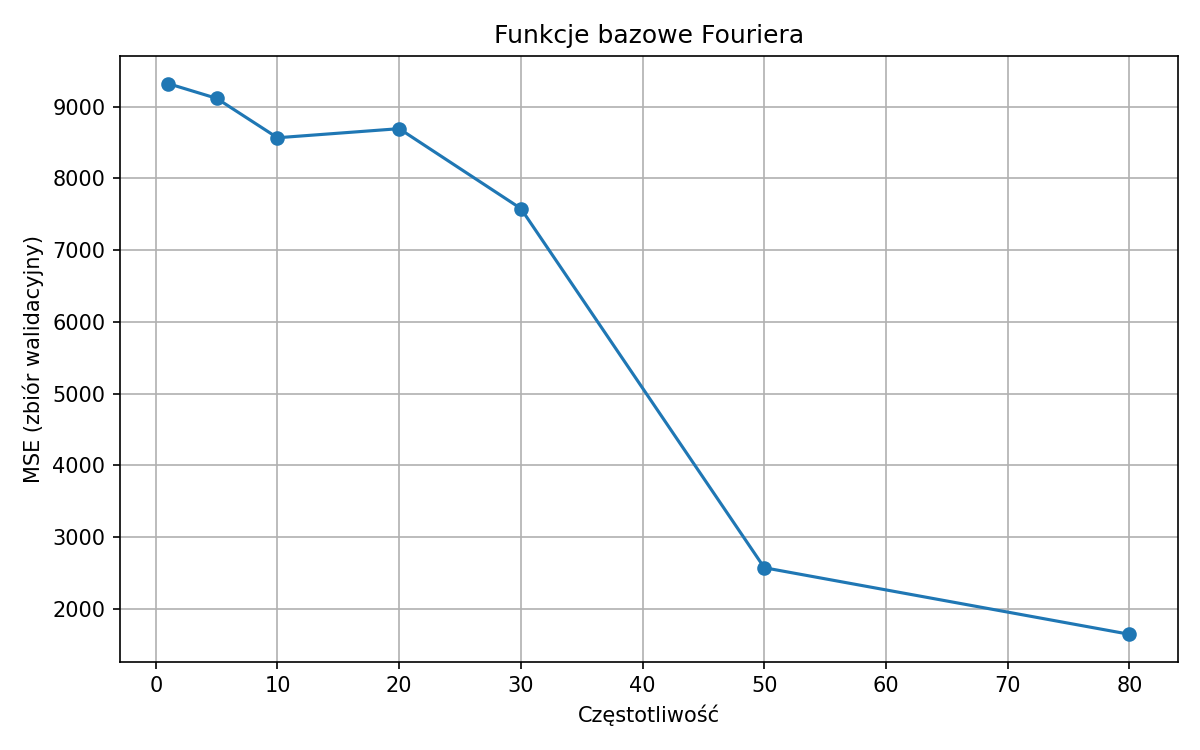
\includegraphics[width=0.55\textwidth]{images/fourier_comparison.png}
    \caption{MSE na zbiorze walidacyjnym dla różnych częstotliwości Fouriera}
\end{figure}

Fourier okazał się najlepszą funkcją bazową -- Test MSE: \textbf{1621.60}.

\subsection{Funkcje sigmoidalne}

Testowałem też sigmoidy $\frac{1}{1 + e^{-(x-\mu)/\sigma}}$ z różnymi parametrami $\sigma$.

\begin{figure}[H]
    \centering
    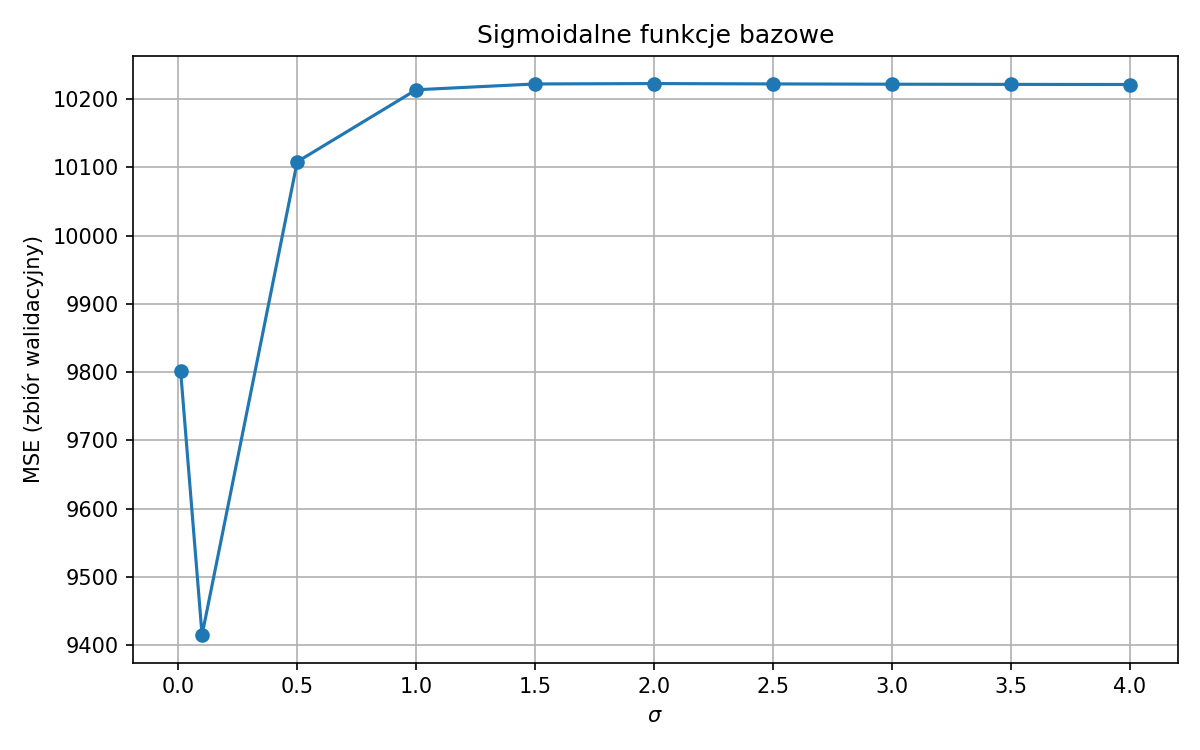
\includegraphics[width=0.55\textwidth]{images/sigmoid_comparison.png}
    \caption{MSE na zbiorze walidacyjnym dla różnych $\sigma$ sigmoidy}
\end{figure}

Sigmoid wypadł najsłabiej -- Test MSE: \textbf{10389.92}. Najwyraźniej sigmoidy nie dodają wiele ponad zwykłe cechy liniowe dla tych danych.

\subsection{Porównanie funkcji bazowych}

\begin{table}[H]
\centering
\begin{tabular}{lr}
\toprule
Funkcja bazowa & Test MSE \\
\midrule
Liniowa & 11440.03 \\
Wielomian (st.~5) & 4942.57 \\
Gaussian ($\sigma = 0.5$) & 4042.12 \\
Fourier (freq = 80) & \textbf{1621.60} \\
Sigmoid ($\sigma = 0.1$) & 10389.92 \\
\bottomrule
\end{tabular}
\caption{Porównanie Test MSE dla różnych funkcji bazowych}
\end{table}

Fourier wygrywa zdecydowanie. Wielomian i gaussowskie też dają dużą poprawę. Sigmoid praktycznie nic nie wnosi.

\section{Krzywe uczenia}

Sprawdziłem jak model radzi sobie na różnych frakcjach zbioru treningowego: 0.01, 0.02, 0.03, 0.125, 0.625, 1. Wyniki uśredniłem po 10 przebiegach z losowym podziałem danych.

\begin{figure}[H]
    \centering
    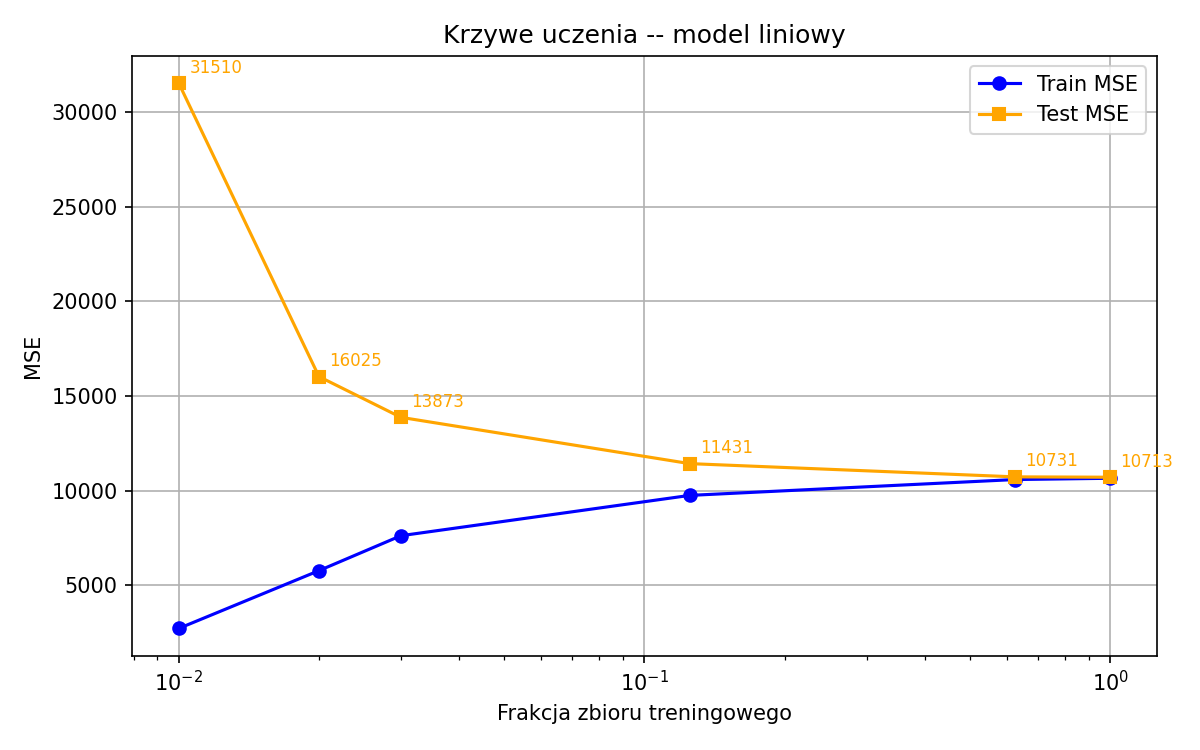
\includegraphics[width=0.7\textwidth]{images/learning_curves_linear.png}
    \caption{Krzywe uczenia dla modelu liniowego}
\end{figure}

\begin{figure}[H]
    \centering
    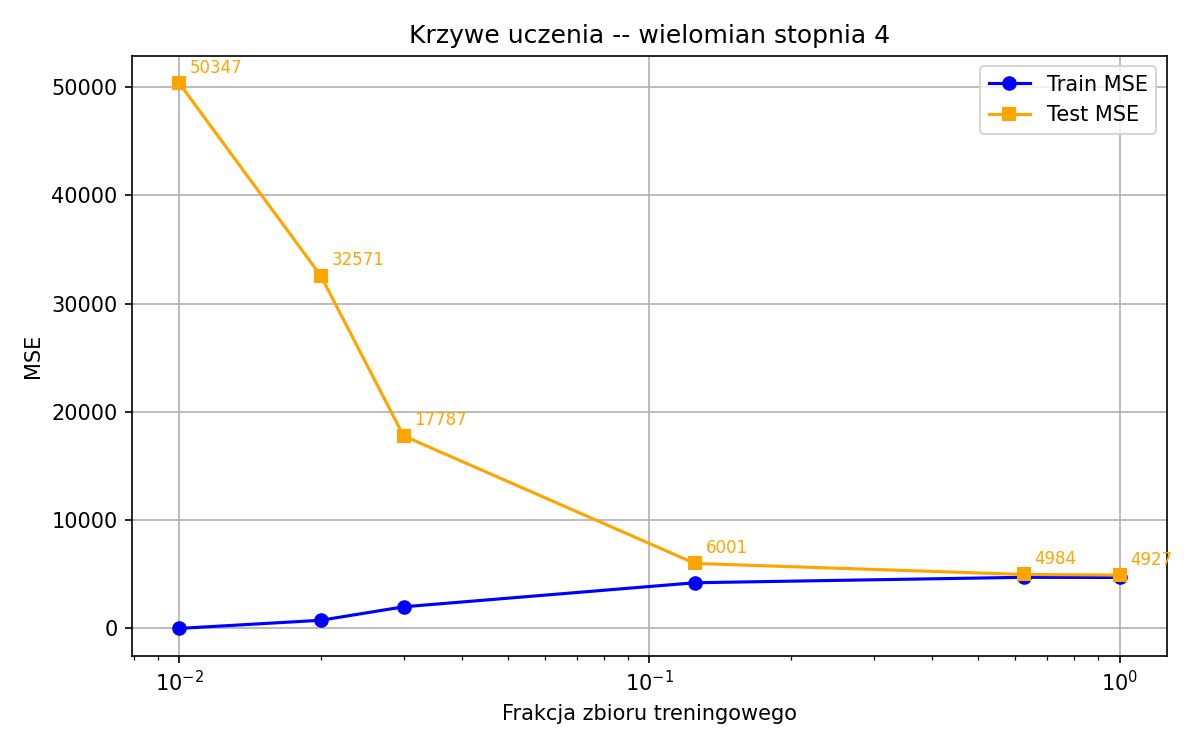
\includegraphics[width=0.7\textwidth]{images/learning_curves_poly4.png}
    \caption{Krzywe uczenia dla wielomianu stopnia 4}
\end{figure}

Przy małej ilości danych model treningowy ma niskie MSE (overfitting), a testowe jest ogromne. Wraz ze wzrostem danych treningowe MSE rośnie, a testowe spada -- krzywe zbiegają się. Model wielomianowy przy pełnym zbiorze treningowym osiąga znacznie lepsze wyniki niż liniowy.

\section{Implementacja}

Cały projekt zaimplementowałem modularnie w Pythonie:
\begin{itemize}
    \item \texttt{src/data.py} -- wczytywanie danych i podział na zbiory
    \item \texttt{src/scaler.py} -- standaryzacja (StandardScaler)
    \item \texttt{src/functions.py} -- funkcje bazowe (Linear, Polynomial, Gaussian, Fourier, Sigmoid, Combined)
    \item \texttt{src/loss.py} -- funkcje straty (kwadratowa, bezwzględna) z regularyzacją
    \item \texttt{src/model.py} -- model regresji (analytical, GD, mini-batch)
    \item \texttt{src/plots.py} -- wykresy
    \item \texttt{src/utils.py} -- krzywe uczenia
\end{itemize}

Klasa \texttt{Combined} pozwala łączyć różne funkcje bazowe, np. \texttt{Combined([Linear(), Gaussian(0.5)])} daje cechy liniowe + gaussowskie.

\section{Podsumowanie}

\begin{itemize}
    \item Prosty model liniowy daje MSE $\approx$ 11440 -- przyzwoite, ale daleko od ideału.
    \item Regularyzacja L1/L2 przy modelu liniowym niewiele zmienia -- model nie overfituje.
    \item Funkcje bazowe najwięcej poprawiają: wielomiany zbijają MSE do $\sim$4943, gaussowskie do $\sim$4042, a Fourier aż do $\sim$\textbf{1622}.
    \item Mini-batch GD działa porównywalnie z pełnym GD, ale jest znacznie szybszy.
\end{itemize}

Najlepszy model to regresja z funkcjami bazowymi Fouriera (połączonymi z liniowymi), osiągający Test MSE $\approx$ \textbf{1621.60}.

\end{document}
